\documentclass[conference]{IEEEtran}

% -----------------------------------------------
%  Packages
% -----------------------------------------------
\usepackage{cite}
\usepackage{amsmath,amssymb,amsfonts}
\usepackage{algorithmic}
\usepackage{graphicx}
\usepackage{textcomp}
\usepackage{xcolor}
\usepackage{booktabs}
\usepackage{multirow}
\usepackage{array}
\usepackage{url}
\usepackage{float}

% -----------------------------------------------
%  Document
% -----------------------------------------------
\begin{document}

\title{Generating Test Scripts for Flutter Applications\\
       Using Pairwise Testing Technique}

\author{
  \IEEEauthorblockN{Titi Changpoo}
  \IEEEauthorblockA{
    \textit{Department of Computer Engineering}\\
    \textit{Faculty of Engineering, Chulalongkorn University}\\
    Bangkok, Thailand\\
    titi.changpoo@gmail.com
  }
  \and
  \IEEEauthorblockN{Taratip Suwannasart}
  \IEEEauthorblockA{
    \textit{Department of Computer Engineering}\\
    \textit{Faculty of Engineering, Chulalongkorn University}\\
    Bangkok, Thailand\\
    taratip.s@chula.ac.th
  }
}

\maketitle

% -----------------------------------------------
\begin{abstract}
% -----------------------------------------------
In the software development lifecycle, unit testing is a critical process
for identifying and resolving defects, thereby enhancing software
reliability prior to delivery. This is particularly crucial in the rapidly
evolving domain of mobile applications developed with the Flutter framework,
where requirements change frequently. Although automated testing reduces
overall testing time, developers still require specialized knowledge and
significant initial effort to create effective test scripts in the Dart
language. This paper presents an automated tool that streamlines the
generation of Flutter test scripts by importing front-end source files,
extracting widget metadata (keys, validation conditions, and input-handling
types), and producing synthetic test data through a Large Language Model
(LLM). Test cases are systematically generated using the Pairwise testing
technique via the PICT tool. The resulting Dart test scripts are ready to
execute within the Flutter testing framework. The tool was evaluated against
three real-world mobile applications---a medical appointment system, a job
listing application, and a real-estate listing application---and achieved
satisfactory branch and line coverage in all cases, demonstrating the
practical effectiveness of the proposed approach.
\end{abstract}

\begin{IEEEkeywords}
Flutter, automated test generation, pairwise testing, Dart, large language
model, mobile application testing, PICT
\end{IEEEkeywords}

% ===============================================
\section{Introduction}
% ===============================================

The global software industry continues to grow rapidly, driven by increasing
demand for mobile applications that are complex, feature-rich, and subject to
frequent requirement changes. Ensuring software quality through comprehensive
testing is therefore essential, yet designing test cases manually is
time-consuming and demands deep expertise from developers \cite{b1}.

Within the Flutter framework \cite{b1}, developers write integration and
widget test scripts in Dart to simulate user interactions on the user interface (UI). However,
crafting these scripts requires developers to (1) understand widget structure
and validation rules in the source code, (2) define appropriate input data
covering valid and invalid boundary conditions, and (3) sequence test actions
correctly. Existing automation tools such as Robot Framework and Playwright
are tailored for web applications and cannot directly generate Flutter-specific
test scripts.

This paper addresses these challenges by proposing an automated tool that:
\begin{itemize}
  \item Parses Flutter front-end (\texttt{.dart}) files to extract widget
        metadata;
  \item Uses a Large Language Model (LLM) (Google Gemini) to synthesize realistic test data;
  \item Applies the Pairwise testing technique through PICT to minimize the
        number of test cases while maximising input-combination coverage;
  \item Outputs executable Dart test scripts ready for the Flutter testing
        framework.
\end{itemize}

The remainder of this paper is organized as follows. Section~II reviews
related work. Section~III describes the proposed methodology. Section~IV
discusses tool design. Section~V presents evaluation results, and Section~VI
concludes the paper.

% ===============================================
\section{Related Work}
% ===============================================

\subsection{Flutter Testing}
Flutter \cite{b1} is Google's open-source UI toolkit for building
cross-platform applications from a single Dart codebase. The framework
provides the \texttt{flutter\_test} library, which exposes a
\texttt{WidgetTester} application programming interface (API) and a rich set of Finders (\texttt{find.byKey},
\texttt{find.byType}, etc.) for locating and interacting with widgets during
testing.

\subsection{Test-Script Generation from Front-End Files}
Ekakrachawakitti \cite{b2} proposed a method for generating Robot Framework test
scripts from web front-end files by extracting HTML elements and input
constraints from a database schema. Srivichayanun \cite{b3} extended this concept
by importing XML Schema Definition (XSD) schemas and applying Boundary Value Analysis to produce test
data for web applications. These works motivate adapting similar extraction
techniques to Flutter's Dart-based widget structure.

\subsection{LLM-Based Data Generation}
Tuan Pham \cite{b4} demonstrated that structuring LLM prompts with distinct
components---context, persona, objective, action, format, and
refinement---significantly improves the quality of generated outputs. This
prompt-engineering strategy is adopted in the present work to drive synthetic
test-data generation.

\subsection{Pairwise Testing}
Pairwise (all-pairs) testing \cite{b7} is a black-box test-design technique
that ensures every pair of input-parameter values is exercised by at least one
test case, dramatically reducing the combinatorial explosion of full coverage.
PICT (Pairwise Independent Combinatorial Testing) \cite{b8} is a widely used
open-source tool that accepts a model file describing parameters and their
levels, and outputs a minimal covering test suite.

% ===============================================
\section{Proposed Methodology}
% ===============================================

The proposed tool automates the end-to-end test-script generation process
through four sequential phases, as illustrated in Fig.~\ref{fig:overview}.

% --- FIGURE 1: Overview ---
\begin{figure}[!t]
  \centering
  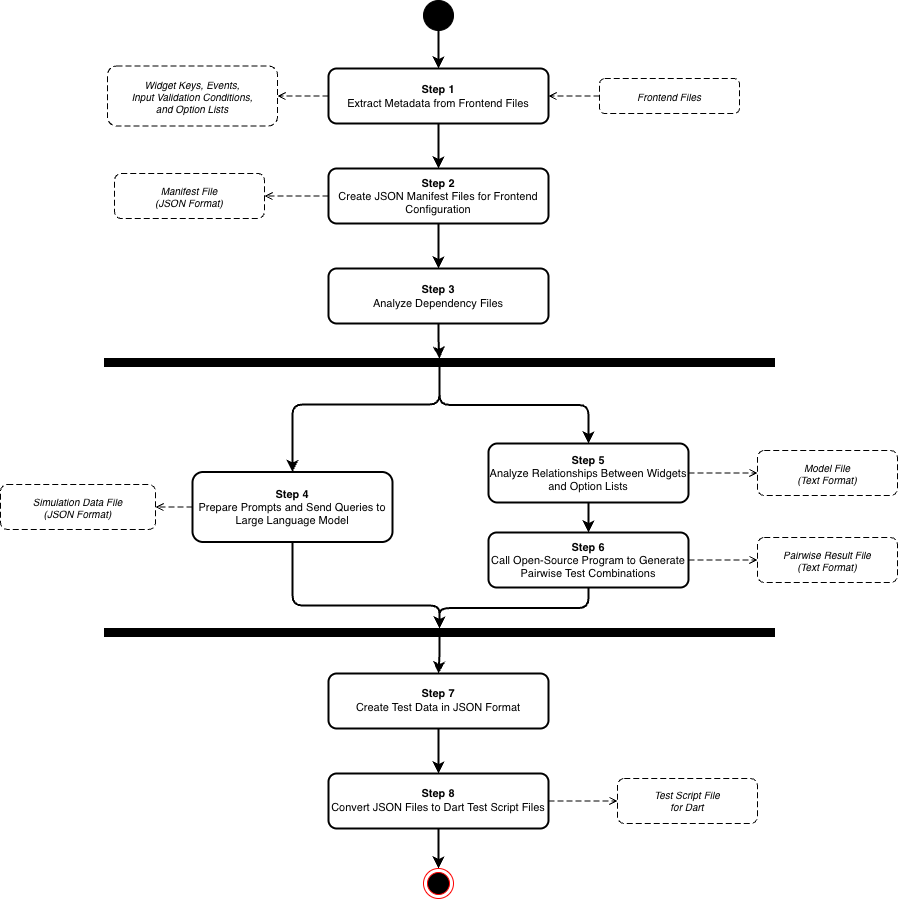
\includegraphics[width=\columnwidth]{figure1.png}
  \caption{Overview of the automated test-script generation pipeline.}
  \label{fig:overview}
\end{figure}

\subsection{Phase 1 -- Extract Manifest}

The tool statically analyzes every \texttt{.dart} file under the
\texttt{lib/} directory of the target Flutter project. Only widgets that
carry a \texttt{Key} property are considered, as the key is required to
locate a widget during test execution via \texttt{find.byKey()}.

For each discovered widget the tool records: (i)~the unique widget key,
(ii)~the widget class name, (iii)~the input type (text, numeric, boolean,
enumerated), (iv)~validation rules parsed from \texttt{validator} or
\texttt{onChanged} callbacks (e.g., required, minLength, regex pattern,
numeric range), and (v)~the selectable options list for
\texttt{DropdownButtonFormField} and \texttt{Radio} widgets.

The extracted metadata is serialized into a \texttt{manifest.json} file
grouped by screen name. Table~\ref{tab:manifest} lists the fields recorded
per widget.

\begin{table}[!t]
  \caption{Metadata Fields in the Manifest File}
  \label{tab:manifest}
  \centering
  \renewcommand{\arraystretch}{1.3}
  \begin{tabular}{ll}
    \toprule
    \textbf{Field} & \textbf{Description} \\
    \midrule
    \texttt{key}         & Unique Flutter widget key \\
    \texttt{widgetType}  & Widget class name \\
    \texttt{inputType}   & Data type: text, number, bool, enum \\
    \texttt{validations} & Parsed validation rules (required, regex, etc.) \\
    \texttt{options}     & Enumerated choices for Radio / Dropdown \\
    \bottomrule
  \end{tabular}
\end{table}

\subsection{Phase 2 -- Generate Datasets}

Given the manifest, the tool constructs a structured LLM prompt following
the CO-STEP (Context, Objective, Scenario, Task, Example, Polish) framework \cite{b4},
which organizes the prompt into five
sections: \textit{context} (describes the Flutter screen under test),
\textit{persona} (instructs the model to act as a QA engineer),
\textit{objective} (requests realistic test data for each widget),
\textit{action} (specifies the generation procedure), and
\textit{format} (enforces a JavaScript Object Notation (JSON) output schema).

The prompt is submitted to \textit{Google Gemini gemini-2.5-flash}
\cite{b5} via the Gemini API. The model returns a
\texttt{datasets.json} file containing, for each widget field, a set of
\textit{valid} values (conforming to all validation rules), a set of
\textit{invalid} values (violating at least one rule), and the
corresponding expected validation outcome. For \texttt{Dropdown} and
\texttt{Radio} widgets, the LLM-generated values are merged with the
option list extracted in Phase~1 to ensure full enumeration coverage.

\subsection{Phase 3 -- Generate Test Data}

Using the datasets, the tool constructs a PICT model file in which each
non-button widget maps to one \textit{factor} and each distinct value maps
to one \textit{level}. Three model variants are built independently:
\begin{enumerate}
  \item \textbf{Valid/Invalid (VI):} factors contain both valid and invalid
        levels; PICT ensures every valid--invalid pair is covered.
  \item \textbf{Valid-only (V):} factors contain valid levels only; PICT
        produces positive-path test cases.
  \item \textbf{Edge:} three manually crafted boundary-value combinations
        (empty input, maximum-length, special characters) are appended.
\end{enumerate}

PICT is invoked as a subprocess with the model file as input. Its
tab-delimited output---one row per test case---is parsed and each row is
mapped to a structured JSON object that records, for every widget: the
widget key, the assigned value, the expected outcome
(\texttt{pass}/\texttt{fail}), and the \texttt{WidgetTester} interaction
command (\texttt{enterText} for \texttt{TextFormField};
\texttt{tap} for \texttt{Radio}, \texttt{Checkbox}, \texttt{Switch}, and
\texttt{ElevatedButton}; sequential \texttt{tap} for
\texttt{DropdownButtonFormField}). The collected rows constitute the
\texttt{testdata.json} file.

\subsection{Phase 4 -- Generate Test Script}

The \texttt{testdata.json} is rendered into a syntactically valid Dart test
file. Each JSON row becomes one independent \texttt{testWidgets} block
structured as follows:
\begin{enumerate}
  \item \textbf{Setup:} the target screen widget is pumped into the test
        environment with \texttt{tester.pumpWidget()}.
  \item \textbf{Interact:} for each widget in the test case, the
        appropriate \texttt{WidgetTester} command is emitted (e.g.,
        \texttt{tester.enterText(find.byKey(Key(`k')), value)}).
  \item \textbf{Assert:} validation-error messages or success indicators
        are verified with \texttt{expect(find.text(`msg'), findsOneWidget)}.
\end{enumerate}
The \texttt{ElevatedButton} widget is always tapped last to trigger form
submission, after which the assertion checks whether the expected outcome
matches the actual UI state.

% ===============================================
\section{Tool Design and Implementation}
% ===============================================

\subsection{Architecture}
The tool adopts a client--server architecture. The back end is implemented as
a \textbf{FastAPI} (v0.114.1) service running inside a \textbf{Docker}
(v28.0.0) container, exposing REST endpoints for each pipeline step. The
front end is a desktop graphical user interface (GUI) application that guides the user through three
inputs: (1) the Flutter front-end file(s), (2) an optional condition JSON
file for custom validation rules, and (3) an output directory path.

\subsection{User Interface}
Fig.~\ref{fig:ui_main} shows the main window of the tool. Users import the
Flutter source file, optionally supply a condition file, and click
\textit{Generate} to trigger the full pipeline.

% --- FIGURE 2: Main UI ---
\begin{figure}[!t]
  \centering
  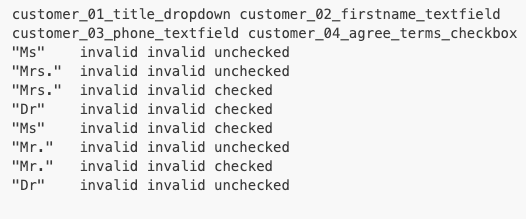
\includegraphics[width=\columnwidth]{figure2.png}
  \caption{Main window of the automated test-script generation tool.}
  \label{fig:ui_main}
\end{figure}

\subsection{Supported Widgets}
The current version supports seven widget types. Table~\ref{tab:widgets}
lists each widget together with its PICT role, the \texttt{WidgetTester}
interaction command used in the generated test, and whether the widget acts
as a PICT factor or is handled as a fixed trigger.

\begin{table}[!t]
  \caption{Supported Flutter Widgets and Generated Test Interactions}
  \label{tab:widgets}
  \centering
  \footnotesize
  \renewcommand{\arraystretch}{1.3}
  \begin{tabular}{p{2.9cm}p{2.3cm}p{1.8cm}}
    \toprule
    \textbf{Widget} & \textbf{PICT Role} & \textbf{Test Command} \\
    \midrule
    \texttt{TextFormField}           & Factor (N levels) & \texttt{enterText} \\
    \texttt{DropdownButton}\newline\texttt{FormField} & Factor (enum) & \texttt{tap} $\times$2 \\
    \texttt{Radio}                   & Factor (enum)     & \texttt{tap} \\
    \texttt{Checkbox}                & Factor \{on,off\} & \texttt{tap} \\
    \texttt{Switch}                  & Factor \{on,off\} & \texttt{tap} \\
    \texttt{ElevatedButton}          & Trigger (fixed)   & \texttt{tap} (last) \\
    \texttt{Text}                    & Assertion target  & \texttt{find.text} \\
    \bottomrule
  \end{tabular}
\end{table}

\subsection{PICT Model Construction}
For a screen with $n$ non-button widgets, the PICT model file contains $n$
parameter lines of the form \texttt{<key>: v1, v2, \ldots, vk}, where each
$v_i$ is a distinct value level. The tool builds three separate model
files---VI, V, and Edge---and invokes PICT once per file. Each PICT run
returns a minimal covering array; the three arrays are concatenated to form
the complete test suite for the screen. For a \texttt{TextFormField} with
five LLM-generated values (three valid, two invalid), the corresponding
PICT factor has five levels. \texttt{DropdownButtonFormField} and
\texttt{Radio} factors enumerate all available options extracted from the
source code.

\subsection{Implementation Constraints}
Each generated script covers \emph{one} application screen per execution.
Every target widget must carry a unique \texttt{Key} property; widgets
without a key are silently skipped. The LLM call uses the Gemini API and
requires an API key at runtime. PICT must be installed on the host system
and accessible on the \texttt{PATH}.

% ===============================================
\section{Evaluation}
% ===============================================

\subsection{Experimental Setup}
The tool was evaluated on three real-world Flutter applications: a
\textit{Medical Appointment} app, a \textit{Job Listing} app, and a
\textit{Real-Estate Listing} app. Two screens per application were selected,
yielding six screen-level evaluations in total. The test environment used
Flutter~v3.27.3 running on macOS Sequoia~15.4.1. Line coverage was measured
using the Flutter \texttt{--coverage} flag combined with \texttt{lcov} to
filter results to UI page files only.

\subsection{Case Study 1: Medical Appointment Application}
The appointment-booking screen exposes seven input widgets. The tool
generated 52 test cases (28 pairwise valid/invalid, 21 pairwise valid, and 3
edge cases) for the booking screen, and 6 test cases for the lighter search
screen. Fig.~\ref{fig:result_medical} shows an excerpt of the generated Dart
test script and its execution log.

% --- FIGURE 3: Medical test output ---
\begin{figure}[!t]
  \centering
  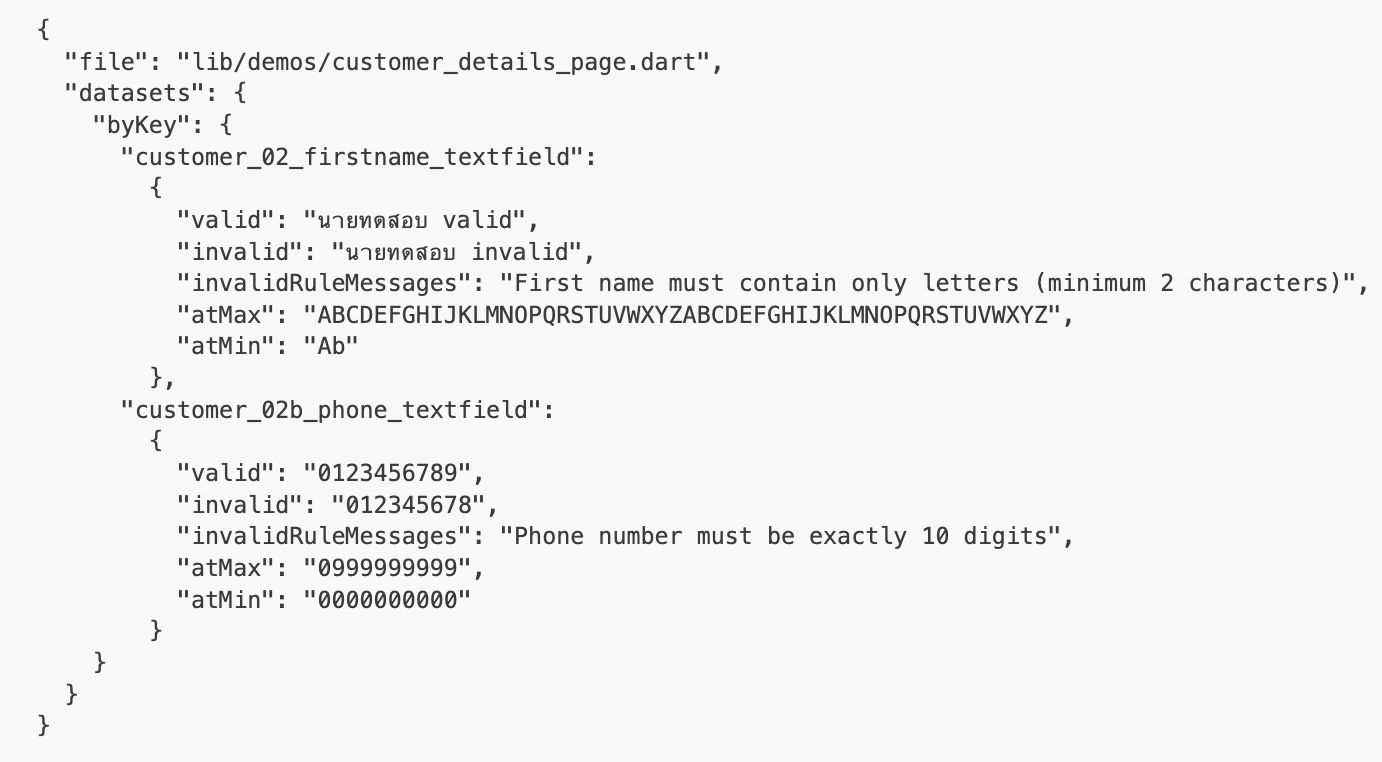
\includegraphics[width=\columnwidth]{figure3.png}
  \caption{Excerpt of the generated test script and execution log for the
           Medical Appointment application.}
  \label{fig:result_medical}
\end{figure}

\subsection{Case Study 2: Job Listing Application}
The job-posting screen includes multiple widgets with complex mutual
validation rules between fields (e.g., salary range constraints). The tool
generated 64 test cases for the posting screen (31 pairwise valid/invalid,
30 pairwise valid, 3 edge) and 63 test cases for the search screen (30, 30,
and 3 respectively), demonstrating that pairwise coverage adapts naturally
to screens with higher widget counts.

\subsection{Case Study 3: Real-Estate Listing Application}
Both the posting and search screens of the real-estate application yielded
55 test cases each (27 pairwise valid/invalid, 25 pairwise valid, 3 edge),
reflecting similar widget complexity across the two screens.
Fig.~\ref{fig:result_realestate} shows the coverage report produced after
executing the generated scripts.

% --- FIGURE 4: Real-estate coverage ---
\begin{figure}[!t]
  \centering
  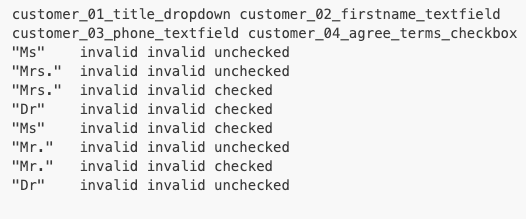
\includegraphics[width=\columnwidth]{figure4.png}
  \caption{Code-coverage report for the Real-Estate Listing application.}
  \label{fig:result_realestate}
\end{figure}

\subsection{Coverage Results}
Table~\ref{tab:coverage} summarises the line coverage and test-case counts
achieved across all six evaluated screens (two per application). Coverage was
measured using the Flutter \texttt{--coverage} flag with \texttt{lcov
--remove} to isolate \texttt{*\_page.dart} UI files from Cubit/State layers.

\begin{table}[!t]
  \caption{Test Coverage Summary}
  \label{tab:coverage}
  \centering
  \renewcommand{\arraystretch}{1.15}
  \begin{tabular}{lcrcc}
    \toprule
    \textbf{Application} & \textbf{Screen} & \textbf{Cases} &
    \textbf{Lines} & \textbf{Coverage} \\
    \midrule
    \multirow{2}{*}{Medical Appt.}
      & Booking  & 52 & 166/173 & 96.0\% \\
      & Search   &  6 & 141/154 & 91.6\% \\
    \midrule
    \multirow{2}{*}{Job Listing}
      & Posting  & 64 & 161/172 & 93.6\% \\
      & Search   & 63 & 223/239 & 93.3\% \\
    \midrule
    \multirow{2}{*}{Real Estate}
      & Posting  & 55 & 169/175 & 96.6\% \\
      & Search   & 55 & 233/250 & 93.2\% \\
    \bottomrule
  \end{tabular}
\end{table}

\noindent All six screens achieved line coverage above 91\%, confirming that
the pairwise-generated test scripts exercise the vast majority of UI code
paths despite the reduced test-case count. Table~\ref{tab:reduction} details
the breakdown of VI, V, and Edge test cases generated per screen.

\begin{table}[!t]
  \caption{Pairwise Test-Case Reduction per Screen}
  \label{tab:reduction}
  \centering
  \renewcommand{\arraystretch}{1.15}
  \begin{tabular}{llccc}
    \toprule
    \textbf{App} & \textbf{Screen} &
    \textbf{VI} & \textbf{V} & \textbf{Edge} \\
    \midrule
    \multirow{2}{*}{Medical Appt.}
      & Booking & 28 & 21 & 3 \\
      & Search  &  2 &  1 & 3 \\
    \multirow{2}{*}{Job Listing}
      & Posting & 31 & 30 & 3 \\
      & Search  & 30 & 30 & 3 \\
    \multirow{2}{*}{Real Estate}
      & Posting & 27 & 25 & 3 \\
      & Search  & 27 & 25 & 3 \\
    \bottomrule
    \multicolumn{5}{l}{\footnotesize VI = pairwise valid/invalid cases;\
    V = pairwise valid cases; Edge = edge cases.} \\
  \end{tabular}
\end{table}

% ===============================================
\section{Conclusion}
% ===============================================

This paper presented an automated tool for generating Flutter widget test
scripts using a combination of source-code metadata extraction, LLM-driven
synthetic data generation, and the Pairwise testing technique. The tool
requires no manual test-case authoring: developers supply only Flutter
front-end files and receive ready-to-run Dart test scripts as output.
Evaluation on three real-world mobile applications confirmed that the tool
successfully generates executable test scripts with measurable code coverage.

Current limitations include support for a fixed set of seven widgets, a
single-screen scope per run, and a dependency on the Gemini API for data
synthesis. Future work will extend widget support, enable multi-screen
scenario testing, investigate alternative open-source LLMs for offline use,
and incorporate feedback loops to refine generated test data based on
execution results.

% -----------------------------------------------
%  References
% -----------------------------------------------
\bibliographystyle{IEEEtran}
\bibliography{references}

\end{document}
